\section{Perceived quality driven tiling scheme}

\subsection{Quality-Bitrate Efficiency}

When we design a tiling method to improve user's perceived quality, we first need to take a look at how client-side optimize perceived quality.

Suppose a video is cut into $T$ tiles and all tiles are of the lowest quality. Bandwidth only allow us to level-up the quality of some of them. So this is a Multiple-Choice Knapsack problem, in which we need to maximize perceived quality with limited bandwidth. In most cases (not always, but with a very high probability) of Multiple-Choice Knapsack problem solutions, item with high performance-cost ratio are more likely to be chosen. Back to our perceived quality optimization problem, the tile with high $\frac{\Delta PSPNR}{\Delta bitrate}$ are more likely to be leveled-up. In other words, when two adjacent tiles with close $\frac{\Delta PSPNR}{\Delta bitrate}$, they are likely to be allocated the same quality level. We can merge these two tiles into a big tile with nearly no bad influence on perceived quality optimization.

So now we make a formal $\frac{\Delta PSPNR}{\Delta bitrate}$ definition. For a client $c$ and a rectangular tile $t$ which can be independently encoded, we define $t$'s \textbf{Quality-Bitrate Efficiency (QBE)} to client $c$ as follow:

\begin{alignat}{2}\
QBE_t^c = \frac{PSPNR_{t_highest}^c - PSPNR_{t_lowest}^c}{B_{t_highest} - B_{t_lowest}} \label{QBE}
\end{alignat}

where $PSPNR_{t_highest}^c$ / $PSPNR_{t_lowest}^c$ denotes the PSPNR value of this tile's highest / lowest bitrate version, and $B_{t_highest}$ / $B_{t_lowest}$ denotes the bitrate of this tile $t$'s highest / lowest bitrate version. 

Suppose server records some view history for a video, a tile's average Quality-Bitrate Efficiency $\hat{QBE}$ can be defined as:

\begin{alignat}{2}\
\hat{QBE_t} = \frac{\sum_1^C{QBE_t^c}}{C} \label{avgQBE}
\end{alignat}

where $C$ is the number of viewer in view history considered into computation.

The formula above has an obvious cold start-up issue. When a video is newly uploaded, there is no view history. $PSPNR_{highest}^c$ / $PSPNR_{lowest}^c$ can not be computed without the information of user behavior. To fix this problem, for videos which don't have enough view history, $PSPNR_{highest}^c$ / $PSPNR_{lowest}^c$ is computed with only consideration of luminance, texture complexity and Depth-of-Field. These informations can be obtained completely on server-side.

\subsection{Tiling video by Quality-Bitrate Efficiency}

Based on above insights, we aim to cut the video into $T$ rectangular tiles of unequal size, such that content items within the same tile have similar $\hat{QBE}$.

In this paper, tiling video by objects consists of 3 steps:

\textbf{Step 1: Partitioning the original video into 12*24 rectangular basic units of equal size.} 

Basic unit is the smallest unit of our tiling method. Each tile must be composed by one or several entire basic units which form a rectangular shape.

\textbf{Step 2: Computing $\hat{QBE}$ of each basic unit.}

We get $\hat{QBE}$ of each basic unit according to (\ref{avgQBE}). After that, suppose a tile $t$ consists of $N_t$ basic units $u_1$, $u_2$, ... , $u_{N_t}$ , we can compute its $\hat{QBE} Variance$ ($QBEV_t$) as follow:

\begin{alignat}{2}\
QBEV_t = \frac{\sum_{1 \le i \le N_{t}}{(\hat{QBE_{u_i}} - E(\hat{QBE_{u_{i}}}))^2}}{N_t}
\end{alignat}

where $E(\hat{QBE{u_i}})$ is the average $\hat{QBE}$ of all basic units in tile $t$:

\begin{alignat}{2}\
E(QBE_{u_i}) = \frac{\sum_{1 \le i \le N_{t}}{QBE_{u_i}}}{N_t}
\end{alignat}

A tile with high QBEV means visual properties (e.g. luminance, texture complexity) of objects in this tile have very different properties. A tile with low QBEV means objects in this tile are similar. So a good tiling scheme should keep each tile's QBEV value as low as possible.

\textbf{Step 3: Merging all basic units into T rectangular tiles and minimize their total QBEV.}

Suppose $V$ is the whole video frame. $R_i$ is the $i$th rectangular tile and $S_i$ is its area.This optimization problem can be formalized as following:

\begin{equation}
\begin{aligned}
\min \sum_{i = 1}^T QBEV_{i} S_i \hspace{3cm} \\
\text{s.t.} \bigcup _{i=1}^N R_{i} = V\hspace{3cm} \\
R_i \bigcap R_j = \emptyset \hspace{1cm} \forall 1 \le i, j \le T
\end{aligned}
\end{equation}

However, this optimization problem is a NP-hard problem, so we can not get the optimal solution in polynomial time. In practice, we apply a dynamic programming algorithm to get the suboptimal solution for this problem. In our implementation, we set $T = 30$ since it performs well in most situations.

\subsection{Comparison of proposed tiling and traditional grid-like tiling}

Fig. \ref{tiling} shows the PSPNR-bandwidth tradeoff of 3*6 grid tiling, 6*12 grid tiling, 12*24 grid tiling and proposed perceived quality driven tiling. 

  \begin{figure}
  \centering
  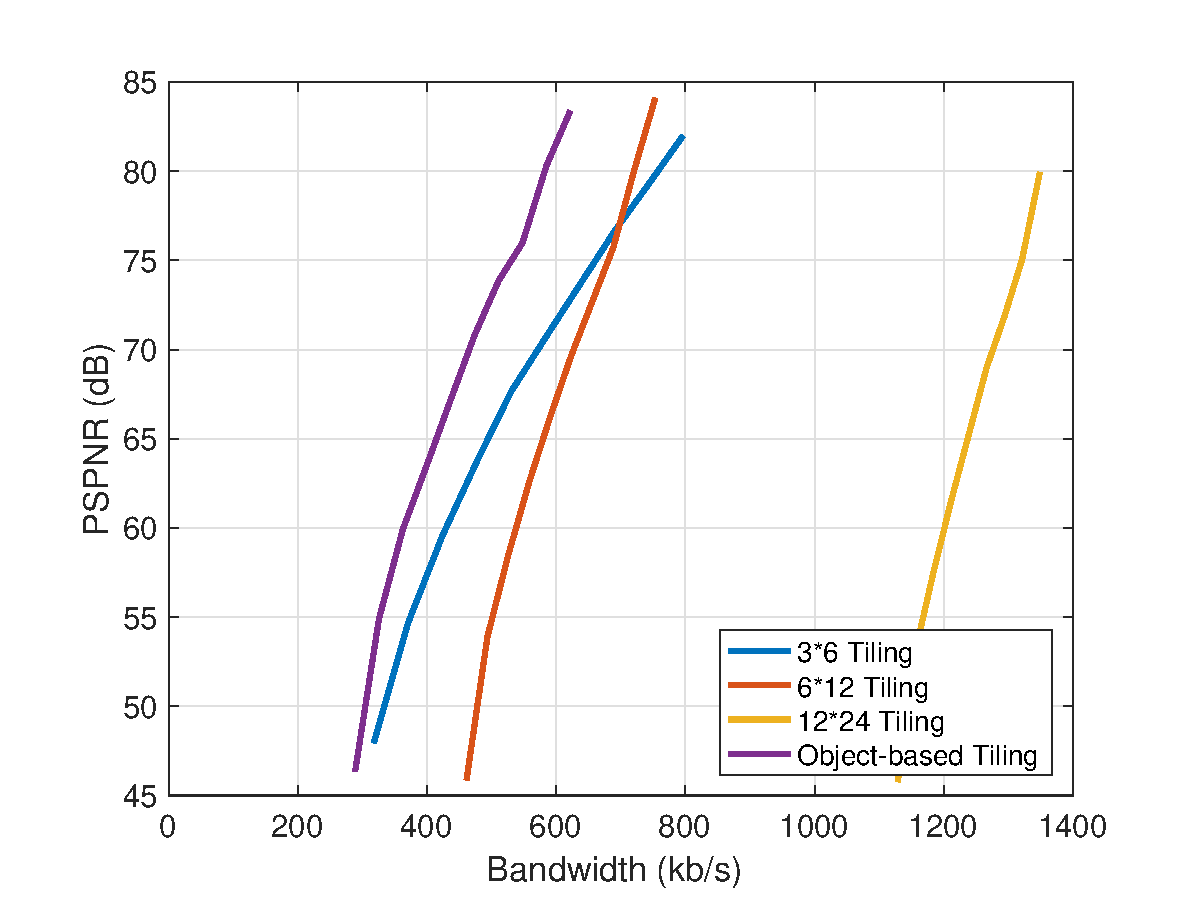
\includegraphics[width=2.5in]{images/tiling.eps}
  \caption{The PSPNR-bandwidth tradeoff of proposed tiling method and traditional grid-like tiling scheme (3*6, 6*12 and 12*24).}
  \label{tiling}
  \end{figure}

For traditional gird-like tiling methods, the performance of different tiling granularity depends on bandwidth. In low bandwidth, most part of video is allocated the lowest bitrate level. So there is no need to cut the video into many tiles. 3*6 tiling performs well because of its high bitrate efficiency. However, in high bandwidth, a coarse tiling granularity causes suboptimal bitrate allocation, so it is beaten by 6*12 tiling. Unfortunately, 12*24 tiling performs poorly in all bandwidth because of its serious bitrate efficiency problem.

Proposed tiling method beats traditional grid-like tiling scheme of all bandwidth. In high bandwidth situation, it saves 20\% bandwidth compared with 6*12 grid-like tiling. Although 3*6 tiling's low bandwidth performance is near to our proposed tiling, its high bandwidth performance is far away from us.
